\documentclass{beamer}
\usepackage{verbatim} % For using /begin{comment}; /end{comment}
%--------------------------------------------------------------%
\setlength{\parindent}{0em}
\setlength{\parskip}{0.5em}
\usepackage{graphicx}
\usepackage{mdwlist}
\definecolor{mine}{RGB}{155,155,155}
\definecolor{oj}{rgb}{1.0,0.65,0.0}
\definecolor{cblue}{rgb}{0.39, 0.58, 0.93}
\definecolor{turq}{rgb}{0.0, 0.81, 0.82}
%\usepackage{caption}
%\captionsetup[figure]{labelformat=empty}

\setbeamercolor{normal text}{bg=black, fg=white}
\setbeamercolor{title}{fg=turq}
\setbeamercolor{frametitle}{fg=oj}
\setbeamercolor{block title}{fg=green}
\setbeamercolor{itemize item}{fg=mine} % all frames will have red bullets
\setbeamercolor{enumerate item}{fg=mine} % all frames will have red bullets

\usefonttheme{serif}
\setbeamerfont{frametitle}{series=\bfseries} % Frame titles should be bold

\title{Basic Principles of Solar Acoustic Holography}
\subtitle{ASTR 500}
\date{11 March 2016}
\author{Laurel Farris}

\begin{document}

\begin{frame}
    \titlepage
\end{frame}

\begin{frame}{Outline}
``Basic Principles of Solar Acoustic Holography''\\
C. Lindsey and D. C. Braun\\
2000
    \begin{enumerate}
        \item Introduction
        \item Basic Principles of Computational Seismic Holography
        \item The Computational Task
        \item Subjacent Vantage Holography
        \item An Example
        \item Acoustic Modelling Based on Holographic Images
        \item Phase-Sensitive Holography
        \item Green's Functions
        \item Summary
    \end{enumerate}
\end{frame}

\begin{frame}{Overview}
    Drawing on principles in optics and optical holography:
    \emph{Observe} the \emph{p}-mode spectrum, and extract
    information without using (possible incorrect) models.

    Comparing:
    \begin{itemize}
        \item simple acoustic-power
        \item phase-sensitive
    \end{itemize}
    Will eventually based solar models off of holographic signatures.

    Propose ``simple computational principles'' to produce images
    from observations.
    
    (Include some sort of eye diagram here?)

\end{frame}

\begin{frame}{1.1}
    ``Seismic holography'' was applied to helioseismic data from SOHO\@.
    ``New'' (1998-1999) solar acoustic phenomena:
    \begin{itemize}
        \item `acoustic moats' surrounding sunspots
        \item `acoustic condensations' 10-20 Mm beneath active regions
        \item `acoustic glories' surrounding complex active regions
        \item first helioseismic images of a flare
    \end{itemize}
    $\rightarrow$ solar cycle dependence of global \emph{p}-modes!
    (which is $\ldots$ ?)

    Magnetic regions reflect \emph{p} modes above the acoustic cutoff
    frequency, where the surface of the \emph{quiet} sun ($\sim$ 10 G)
    acts as a nearly perfect absorber of incident acoustic radiation
    coming from the sun's interior.
\end{frame}

\begin{frame}{1.2 \- The Basic Principle}
    The \emph{phase-coherent} (what does this mean?) computational
    reconstruction of the \emph{acoustic field} in the solar interior,
    so that \emph{stigmatic images} (what are these?) of the sources
    of these disturbances can be produced.

    Historical info here that might go in a pre-paper slide.
\end{frame}

\begin{frame}{1.3}
    \begin{itemize}
        \item Concept proposed in 1975 by Roddier
        \item Developed over the 1990s by Lindsey and Braun
            (current authors)
        \item Key to locating and examining fine structure as deep as
            possible.
    \end{itemize}
\end{frame}

\begin{frame}{1.4}
Seismology and tomography are not the same thing! Tomography is great
for X-ray applications in the medical field, not so good for
astronomical seismology; poor statistics and diffraction limited resolution.
Holography is definitely not just another method of \emph{modeling}
stellar interiors, the images provide more of a basis for modeling
techniques.
\end{frame}

\begin{frame}{1.5}
Helioseismic holography defined in terms of seismic imaging by
phase-coherent reconstruction of the acoustic field into the solar
interior. The terms `seismic imaging' and `helioseismic imaging' are
applied in a broader context to include \emph{partially} coherent
acoustic signatures suggested to appear at the antipodes of far-side
acoustic absorbers. `Holographic' seismology applies to near side, far
side, and everything in between.
\end{frame}

\begin{frame}{Part 2: Basic Principles of Computational Seismic
Holography}
\end{frame}

\begin{frame}{2.1; Figure 1}
    \begin{figure}
        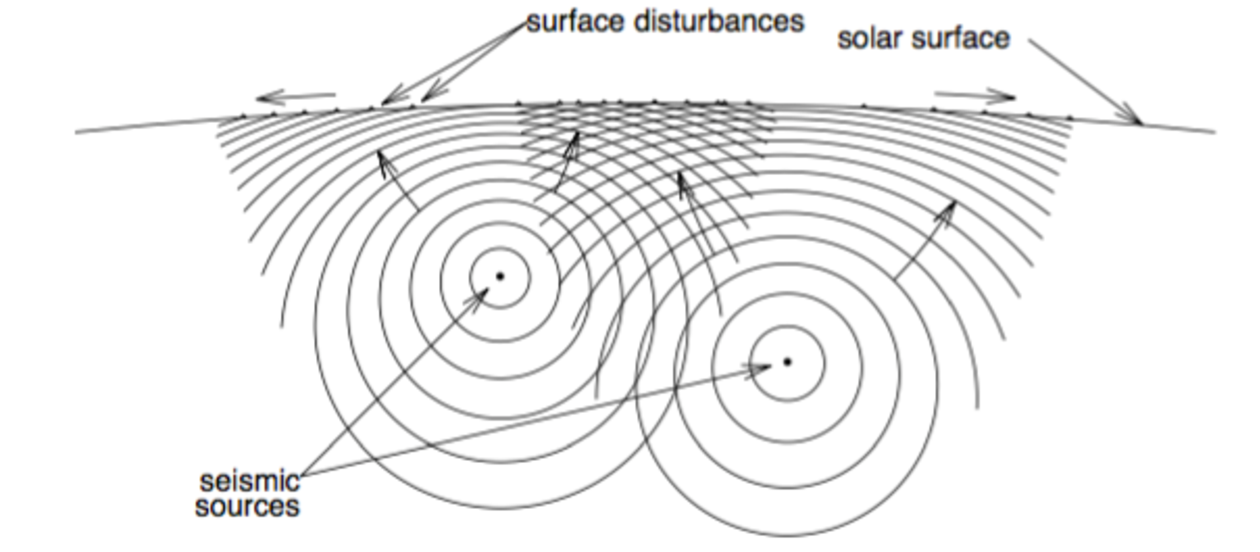
\includegraphics[width=0.8\textwidth]{fig_1.pdf}
    \end{figure}
    \begin{itemize}
        \item Well-defined acoustic sources
        \item All we see is the pattern of ripples at the surface,
            propagating from points directly \emph{above} the sources.
        \item The waves are absorbed upon reaching the surface
            (accurate for $\nu >\ \sim 5.5$ mHz (what's the significance of
            this??)
    \end{itemize}
\end{frame}

\begin{frame}{2.2; Figure 2}
    \begin{figure}
        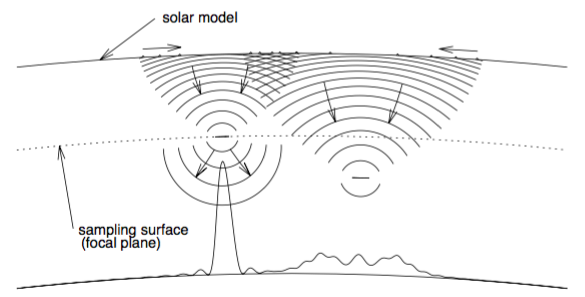
\includegraphics[width=0.8\textwidth]{fig_2.png}
    \end{figure}
    \begin{itemize}
        \item Apply time-series of observations to model with no
            sources, sinks, or scattering (of what?)
        \item The observances are ``seen'' at the ``pupil''.
        \item Place the ``focal plane'' at the location of the
            sources, and get a diffraction-limited signature
            (left side of figure).
        \item If focal plane is above or below the source, we get an
            unfocused, diffuse profile (right side of figure).
    \end{itemize}
\end{frame}

\begin{frame}{2.3; Figure 3}
    \begin{itemize}
        \item Simulation: random acoustic noise in model that
            contains alphanumeric absorbers at six different locations,
            from just below the surface to a depth of 56 Mm
            ($\sim \frac{1}{10}$ R$_{\odot}$).
        \item `acoustic stalactite' of the aborber \- the de-focused
            plume.
        \item a diffuse `stalagmite' appears closer to the absorber
        \item sharp, diffraction-limited silhouette at 56 Mm.
        \item depth diagnostics accomplished by focusing and
        de-focusing, rather than the appearance or disappearance that
        would be used in realistic phyiscal models.
    \end{itemize}
    \begin{figure}
        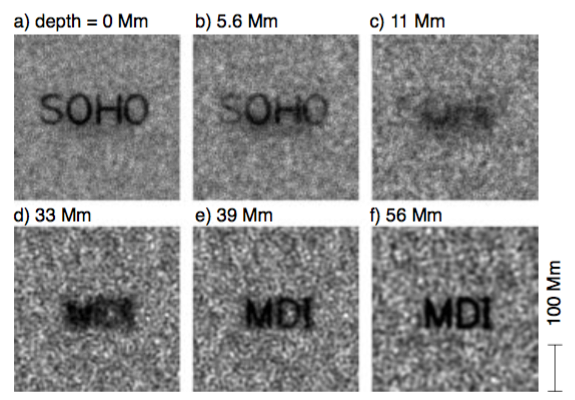
\includegraphics[width=0.8\textwidth]{fig_3.png}
    \end{figure}
\end{frame}

\begin{frame}{2.4}
Seismic holography is most certainly not a representation of solar
acoustics in terms of ray optics. These are mechanical waves, not
electromagnetic ones, though they have similiar behavior, such as
interference and diffraction. Thus, it suffers from the same
limitations as other helioseismological observations, and the same
kind of optimization techniques used to extract information from
coherent electromagnetic radiation can also be used here.
\end{frame}

%-------------------------------------------------------------------%
\begin{frame}{Part 3: The Computational Task}
\end{frame}

\begin{frame}{3.1}
\end{frame}

\begin{frame}{3.2}
\end{frame}

\begin{frame}{3.3}
$$ H_{+}(\mathbf{r},z,t) = \int\textrm{d}t' \int\textrm{d}^{2}r'G_{+}
    (|\mathbf{r}-\mathbf{r}'|,z,t-t')\psi(\mathbf{r}',t')  $$
\end{frame}

\begin{frame}{3.4}
$$ G_{-}(|\mathbf{r}-\mathbf{r'}|,z,t-t')
 G_{+}(|\mathbf{r}-\mathbf{r'}|,z,t'-t) $$

\end{frame}

\begin{frame}{3.5}
\end{frame}

\begin{frame}{3.6}
From the convolution theorem:
$$ \hat{H}_{+}(\mathbf{k},z,\nu) = \hat{G}_{+}(|\mathbf{k}|,z,\nu),
     \hat{\psi}(\mathbf{k},\nu) $$
\end{frame}

\begin{frame}{3.7}
Start getting aberrations; some are easily corrected (e.g.\ spherical
aberration, distortion, and curvature of field). Some however, are not
(coma, primary astigmatism, and higher order aberrations) for large
pupils that are needed to form deep focal planes (deep sources), or
for imaging the far side of the sun. In this case, the
aforementationed wavenumber perspective cannot be used.
\end{frame}

\begin{frame}{3.8}
$$ \check{H}_{+}(\mathbf{r},z,\nu) =
    \int\textrm{d}^{2}r'\check{G}_{+}
    (|\mathbf{r}-\mathbf{r}'|,z,\nu)\check{\psi}(\mathbf{r}',\nu) $$
\end{frame}

%-------------------------------------------------------------------%
\begin{frame}{Part 4: Subjacent Vantage Holography}
\end{frame}

\begin{frame}{4.1}
\end{frame}

\begin{frame}{4.2}
\end{frame}

\begin{frame}{4.3}
\end{frame}

%-------------------------------------------------------------------%
\begin{frame}{Part 5: An Example}
\end{frame}

\begin{frame}{Figure 4}
    \begin{figure}
        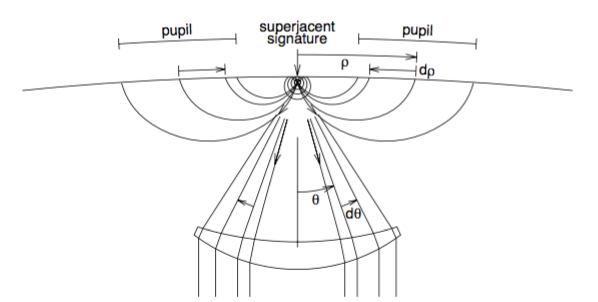
\includegraphics[width=0.8\textwidth]{fig_4.png}
    \end{figure}
\end{frame}

\begin{frame}{Figure 5}
    \begin{figure}
        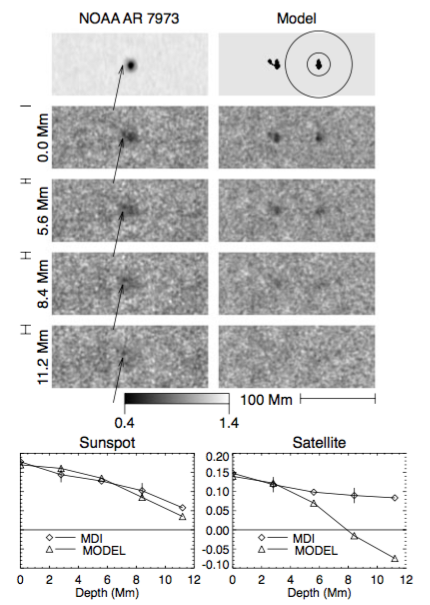
\includegraphics[width=0.8\textwidth]{fig_5.png}
    \end{figure}
\end{frame}

\begin{frame}{Figure 6}
    \begin{figure}
        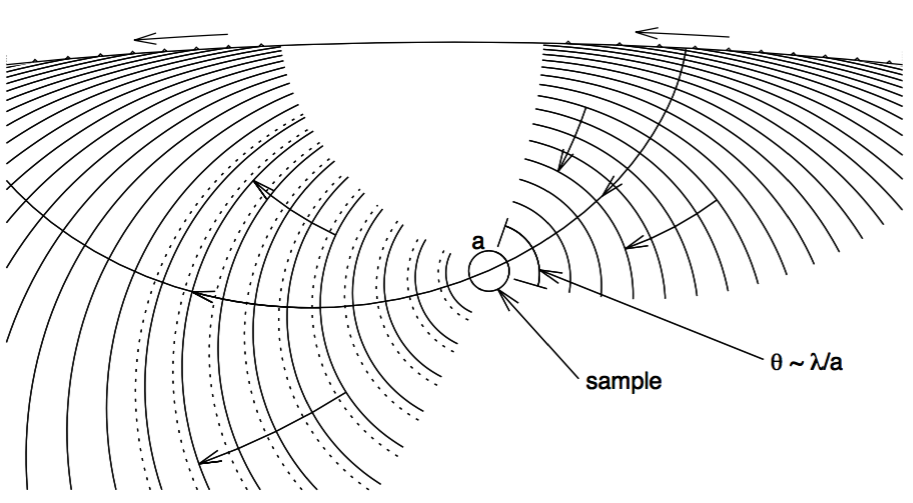
\includegraphics[width=0.8\textwidth]{fig_6.png}
    \end{figure}
\end{frame}

\begin{frame}{Figure 7}
    \begin{figure}
        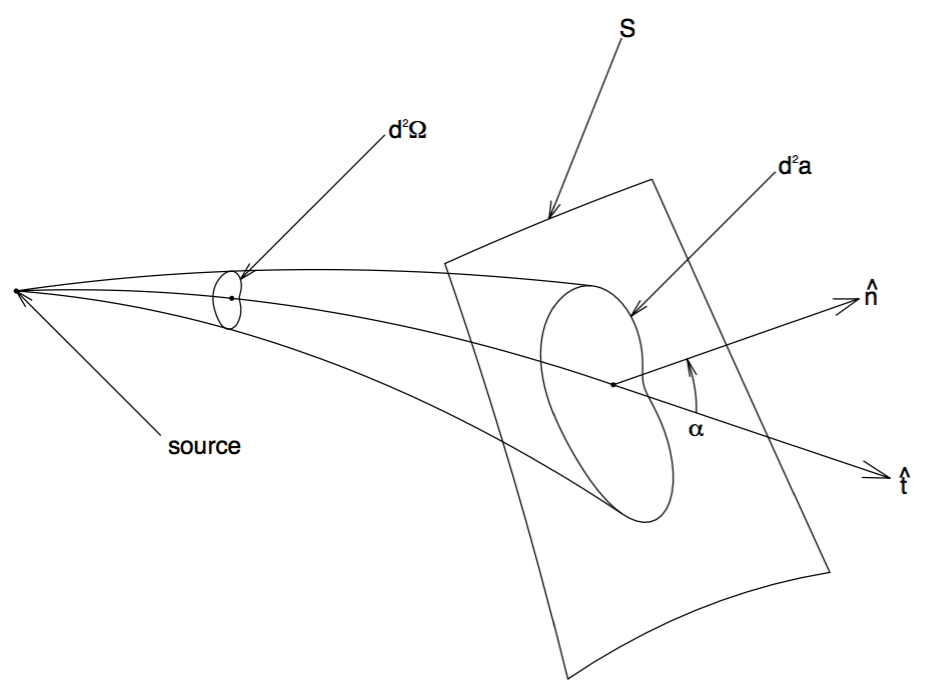
\includegraphics[width=0.8\textwidth]{fig_7.png}
    \end{figure}
\end{frame}

\begin{frame}{Figure 8}
    \begin{figure}
        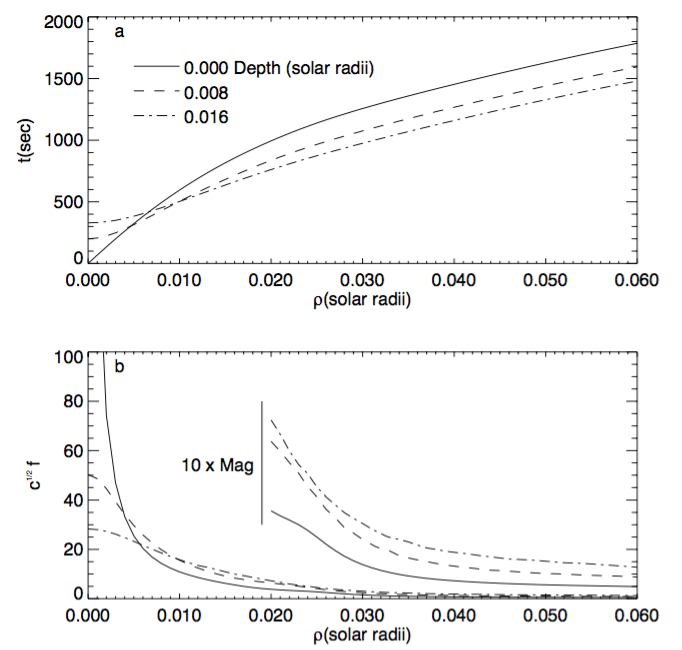
\includegraphics[width=0.8\textwidth]{fig_8.png}
       % \caption{captiontext}
       % \label{figurelabel}
    \end{figure}
\end{frame}

\begin{frame}{Figure 9}
    \begin{figure}
        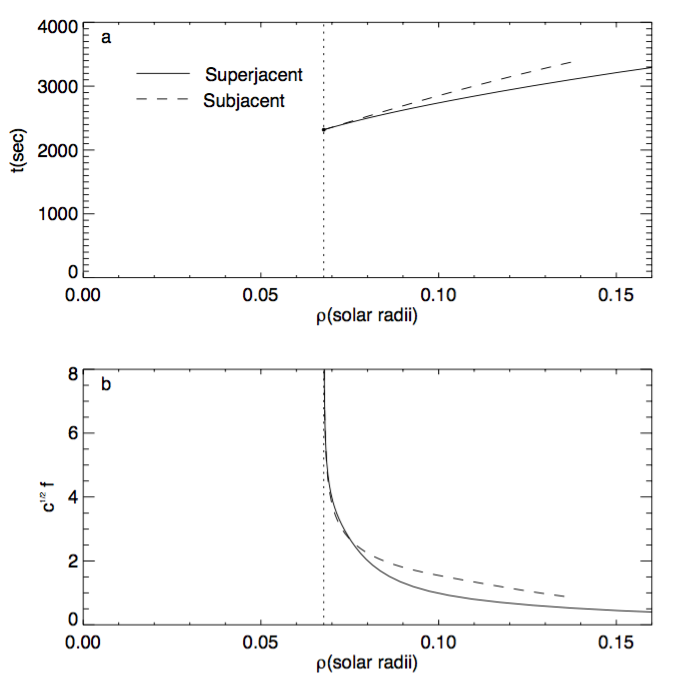
\includegraphics[width=0.8\textwidth]{fig_9.png}
       % \caption{captiontext}
       % \label{figurelabel}
    \end{figure}
\end{frame}

\begin{frame}{Figure 10}
    \begin{figure}
        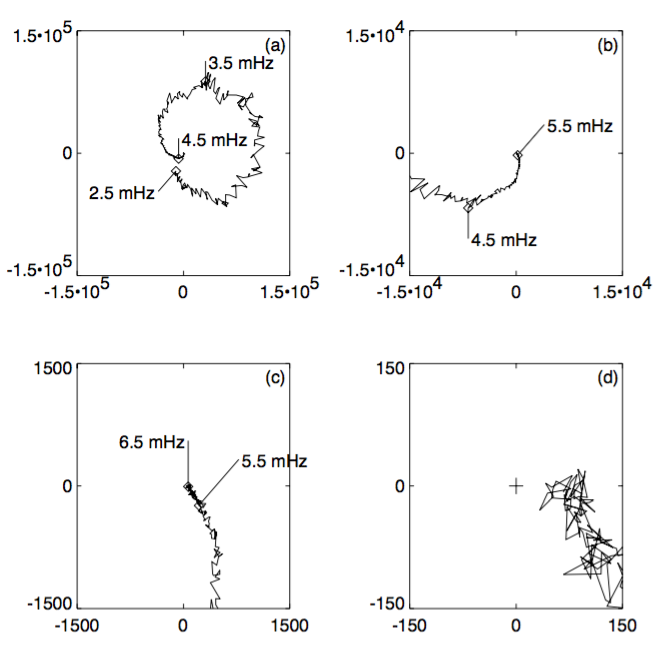
\includegraphics[width=0.8\textwidth]{fig_10.png}
       % \caption{captiontext}
       % \label{figurelabel}
    \end{figure}
\end{frame}

\begin{frame}{Figure 11}
    \begin{figure}
        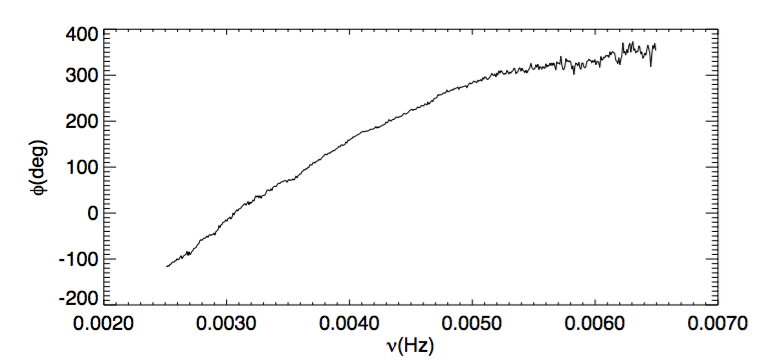
\includegraphics[width=0.8\textwidth]{fig_11.png}
       % \caption{captiontext}
       % \label{figurelabel}
    \end{figure}
\end{frame}

%--------------------------------------------------------------%

\end{document}
